\section{Study 2: Strength Perceptions}
With an observational online study, we explored the associations between psychological variables and password strength perception. As outlined in Chapter \ref{chap:pasdjo}, we regard the perception of strength as an implicit driver for behavior, which is more difficult to observe. Hence, we explored associations between subjective password strength ratings and scores on well-established psychometric scales. 
%task description
The task resembled the PASDJO game: participants were shown a password, and they had to rate it on a seven-point scale. We chose seven point scales to make the approach more comparable to Ur \etal \cite{Ur2016PerceptionsPassword}. Moreover, we gave participants two passwords, and they had to decide which one was stronger. 

%pre-registration
Before we ran the study, we pre-registered the experiment with the open-science framework (OSF)\footnote{\url{https://osf.io/}, last accessed 11.09.2016} and planned to conduct all analyses as predicted to mitigate confirmation bias. However, the envisioned statistical  tests were not always applicable, which forced us to consider more appropriate methods and move away from the pre-registration. Since we consider our research efforts mostly exploratory, we approached the study without specific hypotheses regarding the influence of certain personality traits on the perception of password strength.

\subsection{Structure}
% First Part: DEMOGRAPHICS
The study was divided into six parts. Two parts were standard psychometric tests. We describe all parts, to give the reader the full picture about the participants' tasks. However, we have to omit a few less important results for the sake of clarity. After a brief introduction where the participants were informed about the background of the study, the first step was to provide basic demographic information regarding gender, age, educational and professional background. %This information is important for the ratings on the password scales, because advanced knowledge in IT(-security) may lead to a different rating than the general audience. 

% Second Part: META STATISTICS / CREATION
\paragraph{Meta Password} The second part elicited characteristics about the passwords that our participants used on real online accounts. Here, we asked about typical password attributes, like LUDS (lower-, uppercase, digits, symbols), length and the inclusion of dictionary words. The collection of such password descriptions is an ethically reasonable way to study actual behavior that does not directly involve creating and disclosing an entire password \cite{VonZezschwitz2013SurvivalShortest}. Participants could select from a list of accounts that they used on a regular basis, e.g. Facebook, YouTube, Netflix, Google. If they did not have any of the selectable accounts they could provide another. We call the description of a participant's password on any of these sites ``\textit{meta password}'' in the remainder of the chapter. We included this part in the survey to explore additional covariates for strength perception.
%TODO entscheiden ob das reinkommt Additionally we had them create a password which they would rate as sufficient to protect such an online account and that is memorable. We asked not to enter a password that they were currently using. At the end of the study, we again inquired after the fictional password to measure short-term memorability. 

%%% TABLE: PASSWORDS
\begin{table}[htbp]
  \centering
  \caption{Set of passwords that we divided into different length and strength categories (as measured with zxcvbn). Features: U = uppercase, D = digits, S = symbols}
 % \small
    \begin{tabular}{lllcccr}
    \multicolumn{1}{c}{\multirow{2}[1]{*}{Password}} & \multicolumn{2}{c}{Categories} & \multicolumn{3}{c}{\multirow{2}[1]{*}{Features}} & \multicolumn{1}{c}{guesses} \\
      & Length & Strength & \multicolumn{3}{c}{} & \multicolumn{1}{c}{(log10)} \\
    \midrule
    hagrqqqqthhbbe & Long & Strong & \multicolumn{3}{c}{-} & 12.48 \\
    etuhcarap & Short & Weak & \multicolumn{3}{c}{-} & 4 \\
    AbWxCdYz & Short & Medium & \multicolumn{3}{c}{U} & 8 \\
    1qaz2wsx3edc & Long & Weak & \multicolumn{3}{c}{D} & 3 \\
    a6a4ba8a & Short & Medium & \multicolumn{3}{c}{D} & 8 \\
    ieatkale88 & Short & Medium & \multicolumn{3}{c}{D} & 10 \\
    thedzfhg123 & Short & Medium & \multicolumn{3}{c}{D} & 10 \\
    11Nd1sPPut8ble99 & Long & Strong & \multicolumn{3}{c}{U,D} & 16 \\
    bicycles-peaches-cold & Long & Strong & \multicolumn{3}{c}{S} & 13.69 \\
    AatIcs,ijayl-t & Long & Strong & \multicolumn{3}{c}{U,S} & 13.95 \\
    p@ssw0rd & Short & Weak & \multicolumn{3}{c}{D,S} & 0.95 \\
    ocean4 Size !beer Car & Long & Strong & \multicolumn{3}{c}{U,D,S} & 20.39 \\
    F@m1Ly07\% & Short & Medium & \multicolumn{3}{c}{U,D,S} & 6.88 \\
    \bottomrule
    \end{tabular}%

  \label{tab:password-list}%
  
\end{table}%

% Third Part:  RATING
\paragraph{Standalone Strength Rating} In the third part of the study, the \textit{rating part}, the participants assessed the strength of one password at a time in random order, similar to playing PASDJO. The passwords had to be rated on 7-point scales ranging from \textit{1 = very weak} to \textit{7 = very strong}. We picked a set that was comparable to related work \cite{Ur2016PerceptionsPassword} and that we carefully designed around certain attributes. Table \ref{tab:password-list} shows the selected set of passwords and their features. The ``length'' category distinguishes between short passwords with nine characters or less and long passwords with ten characters or more. The distinction is inspired by real-world policies that most commonly require up to nine characters (see Chapter \ref{chap:policies_reuse}). The ``strength'' category groups passwords on three levels by their guess number as determined by zxcvbn. Weak passwords require less than $10^{6}$ guessing attempts, strong passwords at least $10^{12}$ guesses, and medium passwords anything in between. This classification is in concordance with related work \cite{Florencio2014AdministratorsGuide, Wheeler2016zxcvbn} . To fully counterbalance all category combinations, one would require 120 items, which we could not implement for the sake of brevity. Hence, we kept the number of items small to mitigate fatigue during the study sessions. In the chosen set of 13 passwords, there were at least three items for each distinct category, i.e. three short, long, weak and strong passwords, and at least three passwords pertaining to different LUDS policies (lowercase, uppercase, digits and symbols).

% Fourth Part: COMPARISON
\paragraph{Comparison} Following a similar procedure as Ur et al. \cite{Ur2016PerceptionsPassword}, participants moved on to compare the strength of passwords pairs (\textit{comparsion part}). The 7-point scale ranged from ``<left password> is much stronger'' to ``<right password> is much stronger''. The pairs were constructed such that the passwords differed, e.g., in the existence and positions of digits and uppercase letters. Figure \ref{fig:comparisontask} illustrates our scoring schema. 

\begin{figure}
	\centering
	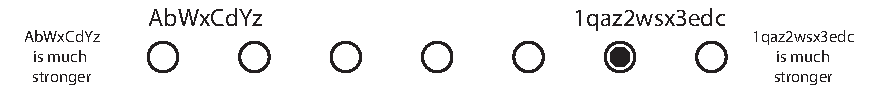
\includegraphics[width=\linewidth]{figures/comparisontask}
	\caption{\label{fig:comparisontask} Simplified item of the comparison task. The passwords differ in length, strength, and the usage of uppercase letters and digits. Here would have scored the importance of length and digits with +2 while the importance of strength and uppercase letters was scored with -2.}
\end{figure}

If the passwords measurably differ in strength as in Figure \ref{fig:comparisontask}, the ratings show if the participants' perceptions match reality. In total, ten comparisons had to be made in random order, in which we permuted the combinations. For this task, we also added an attention check where the passwords on both sides of the scale matched, allowing us to exclude responses where the answer differed from ``both passwords are equally strong''. 

\paragraph{SeBIS} Next, we requested self-assessment about security-related behavior using the Security Behavior Intentions Scale (SeBIS) \cite{Egelman2015SeBIS}. This scale comprises the dimensions \textit{securement}, \textit{passwords}, \textit{awareness}, and \textit{updating}. For each dimension, a score is calculated with four items totaling up to 16 additional items in our study. However, in discussions after the experiment we received hints that it would have been better to include a gap of a couple of days before collecting the SeBIS data to ensure its validity. Since we failed to take this into account beforehand, we do not report the results further, but it is important to mention that the questionnaire included those 16 items. 
%The items are phrased as statements to which respondents can indicate how often they show a certain type of security-related behavior. The scale ranges from \textit{1 = never} to \textit{5 = always}. The \textit{password} dimension measures general attitude towards passwords, which we can utilize to inform our interpretation later.

\paragraph{Big Five} The study concluded with two psychometric tests. In the \textit{Big-Five part}, we utilized a set of 50-items from the International Personality Item Pool (IPIP), which is a representation of Costa and McCrae's NEO-PI-R domains \citep{Costa1992NEO}\footnote{All items of the personality test can be found here: \url{http://ipip.ori.org/newNEODomainsKey.htm}, psychometric properties: \url{http://ipip.ori.org/newNEO_DomainsTable.htm}}. In this personality test, participants rate how accurately a certain statement portraying a certain personality characteristic describes themselves. Each item is a 5-point scale with the labels \textit{very inaccurate, moderately inaccurate, neither accurate nor inaccurate, moderately accurate, very accurate}. Every personality trait is tested with five positively and five negatively keyed items. It was shown that the 50-item version of the test shows high correlation with more exhaustive tests ($r > 0.75$ in all dimensions) and is thus a sufficiently reliable test. We randomized the order of the items.

\paragraph{GDMS} Egelman and Peer found that the general decision-making style had higher predictive power than the Big-Five traits for privacy-related behavior \cite{Egelman2015AverageUser}. Thus, we wanted to test the feasibility of both psychometric tests and finished the study with the \textit{GDMS part}. This scale uses 25 positively keyed items to measure the five decision-making styles \textit{rational}, \textit{intuitive}, \textit{dependent}, \textit{avoidant} and \textit{spontaneous}. 



\subsection{Quantitative Analysis}
Since at least three passwords showed a certain characteristic, e.g. uppercase letters, we averaged the ratings for them accordingly and used them as dependent variables. Moreover, in the psychometric tests we accounted for negatively keyed items, i.e. those items that were phrased with negations like \textit{``I don't talk a lot''}. We inverted the ratings where necessary and afterwards calculated the sum of agreement levels for each dimension (\textit{trait score}). 

%cleaning the data
As in Section \ref{sec:personality:study-1}, we repeatedly fit a \gls{GAM} to our data, i.e. a more flexible and interpretable form of regression\footurl{https://multithreaded.stitchfix.com/assets/files/gam.pdf}{06.02.2018}. 
%DV
Subjective password strength assessments, respectively comparisons, serve as dependent/response variables. We calculate one score per participant and password category by adding up the corresponding ratings. For instance, if they rated all eight passwords containing digits with seven points, their score for ``G\_Digits'' (\textbf{G}roup of passwords with digits) is 56. We average participants' ratings for models that require means instead of total scores. 
%Only to compare the means in each password category, we average the ratings. 

%IV
Psychometric scores on all several sub-dimensions served as independent variables (covariates). We always control the regression models for gender, technical background and age to contrast effects. Wherever possible, we model covariates as linear, if the GAM indicates that smoothing is unnecessary. For this data-set, we also conducted principal component analysis followed by factor analysis. The resulting factors are then used to fit additional models for comparison. This allows us to evaluate the suitability of the Big Five inventory for our exploration.
%Since some \gls{GAM} smooth terms might make models worse, we use automatic penalization to basically remove them from the model\footurl{https://www.rdocumentation.org/packages/mgcv/versions/1.8-23/topics/gam.selection}{06.02.2018}. 

%We check for collinearity using variance inflation factors (VIF) and only retain factors with VIFs close to 1 \cite[p. 217]{Weisberg2005applied}. 
%Finally, we perform Durbin-Watson tests to rule out auto-correlation effects (target value $d=2$). While p-values do not add much to the interpretability of the findings, we report them for the sake of completeness.  
%TODO Quelle!
%Our level for statistical significance is $\alpha = 0.05$, unless Bonferroni correction requires a lower value. 

%When we report the results of linear regression models, we only do so for the models with the highest adjusted $R^2$ value, i.e. the model where the number of predictors leads to the best model-fit explaining the variance in the dependent variable. The values in Tables \ref{tbl:personalpw_regression} through \ref{tab:Comparison-Regression} are the \textbf{standardized beta} correlations, i.e. they are unit-less and lie between -1 and +1. 

\subsection{Qualitative Analysis}
To better understand the reasoning behind the ratings and comparisons, we also inquired how the respondents approached the rating task. They could enter free-text answers after all ratings were done. The answers were then coded independently by two members of the team. The first coding step was to find categories and propose the code book. Afterwards, the proposed codes were handed over to the second coder, who sorted answers into the categories and amended new ones where necessary. Interrater agreement between the two coders was satisfactory (78\%, Krippendorff's $\alpha = 0.55$) and the final the code book could be created after discussing the discrepancies. We report how many participants mentioned a particular theme in their response regarding their rating strategies.


\subsection{Recruitment}
We utilized the online research platform Prolific\footnote{\url{https://prolific.ac}, accessed 01.09.2016} to administer our survey. Participants received \$2.65 upon successful completion, which took 20 minutes in average. This compensation level is suggested as part of the ethical reward guidelines on the platform. Only an English-speaking audience was eligible to participate. From the 178 people who started the survey, 104 finished it. To prevent low quality answers, we introduced an attention check during the comparison part of the experiment.  



\subsection{Ethical Considerations}
There is no institutional review board for this kind of studies at our institution. However, we designed the questionnaire to respect the participants' privacy and did our best to minimize the level of disclosure of sensitive data. The metrics we collected to characterize the participants' passwords are most likely insufficient to reconstruct the passwords in a straightforward way and can thus be considered ethically acceptable. 


\subsection{Limitations}
%It is good to discuss the limitations before the results. Thus, the reader can bear them in mind when they are reading on. 

Like most studies involving personality assessment, the result is only a rough model of a person's personality and does not include all facets. We chose a test with 50 items to assess the Big-Five traits. While such psychometric tests exist with item counts between 10 \cite{Gosling2003TIPI} and 240 items \cite{Costa1992NEO}, the 50-item version has high internal reliability and does not fatigue the respondents as much as more exhaustive tests. Additionally, with a sample size of 100 participants, power-analysis tells us, that only strong and medium interactions are likely to be found for with our regression models (cf. \cite{Shevlin1998SampleSize} or \cite[p. 223]{Field2005DiscoveringStatistics}). At this stage of the exploration, however, this is what we aimed for. If we do find effects with such a small sample, then they must be large enough to justify follow-up investigations with larger samples. Moreover, statistical analyses can be done very differently. We traded off model complexity and interpretability to draw first conclusions. Thus, the reported associations can never be seen \textbf{causal effects}, because we would have to use different experimental setups, and carry out the experiments many times on larger samples. In the scope of our personality studies, we therefore provide pointers and possible explanations, but do not claim that the results are highly generalizable. This is especially important, because the sample stems from a technically savvy audience. Users registering for tools like Prolific or Amazon Mechanical Turk may also have stronger financial motivation to do so than the rest of the population \cite{Ross2010WhoAreTurkers}. 

Furthermore, the methodology relies on self-assessment and honest answers, which are difficult to control. We introduced an attention check to mitigate the problem, by asking people to compare two identical passwords. For the meta-password, we do not know whether it was created on a mobile or desktop device. Passwords created on mobiles are usually less complex than those created on desktops \cite{Melicher2016UsabilityMobileTextPasswords, VonZezschwitz2014HoneyIShrunkTheKeys}. 

Finally, the study set-up and procedure may also influence the interpretability of the outcome. We decided not to randomize the order of the question blocks to maintain full control over the general procedure. When we measure dependent variables, the order of questions is still randomized in the question groups. This way, the potential fatigue effects are the same for all participants at the different stages, while the important questions are in random order. Moreover, the items for password pairs were not fully counterbalanced on all levels to prevent fatigue when answering the entire questionnaire. A more exhaustive set of tested passwords would increase the generalizability. 



%%%%%%%%%%%%%%%%%%%%%%%%%%%%%%%%%%%%%%%%%%%
%%%%
%%%%
%%%%			RESULTS 
%%%%
%%%%
%%%%%%%%%%%%%%%%%%%%%%%%%%%%%%%%%%%%%%%%%%%
\subsection{Results}
In this section, we first describe the participants and meta password characteristics before we proceed to the regression analyses. Since we created plenty of regression models, we only report those who showed notable associations -- mostly for ``Overall'' and ``Digits'' in the rating part, and ``Symbols'' and ``Digits'' in the comparison part. We omit results from other psychometric measures (GDMS, SeBIS) for the sake of stringency. The final part of this section shows qualitative findings and a brief synthesis of the results. 

\subsubsection{Participants}
We collected 104 complete samples. We had to remove three samples from respondents who failed the attention check. Another response was removed because all responses on point scales were answered with the same value. This procedure is proposed by the IPIP project\footnote{\url{http://ipip.ori.org/newValidity.htm} accessed 02.09.2016}. The resulting total N = 100 was divided into 42 female and 58 male participants. Their average age was 28 years ($Standard Deviation~(SD) = 9,~Minimum = 16,~Maximum = 61,~Median~(Md) = 26$). 44 responses came from students. The education level was high with 59 participants reportedly having a bachelor's (44) or master's (15) degree. 29 participants claimed to have a computer science or IT-related background. In summary, our sample stems from a young, educated and fairly technically savvy population. This convenience sample is not ideal, but we hope to deal with this skew by including demographics as predictors in the regression models.

\subsubsection{Ratings Descriptives}
On average, the respondents correctly identified weak, medium and strong passwords in the rating task, i.e. their perception matched reality. The average subjective scores were $M=3.60~(SD=1.07)$ for weak, $M=4.25~(SD=0.95)$ for medium and $M=4.71~(SD=0.90)$ for strong passwords. A Friedman rank test showed that these ratings differed significantly ($F(2)=59.91,~p < 0.001$). Figure \ref{fig:personality:study2:average-rating-boxplot} shows all averages per group.

\begin{figure}[htbp]
	\centering
	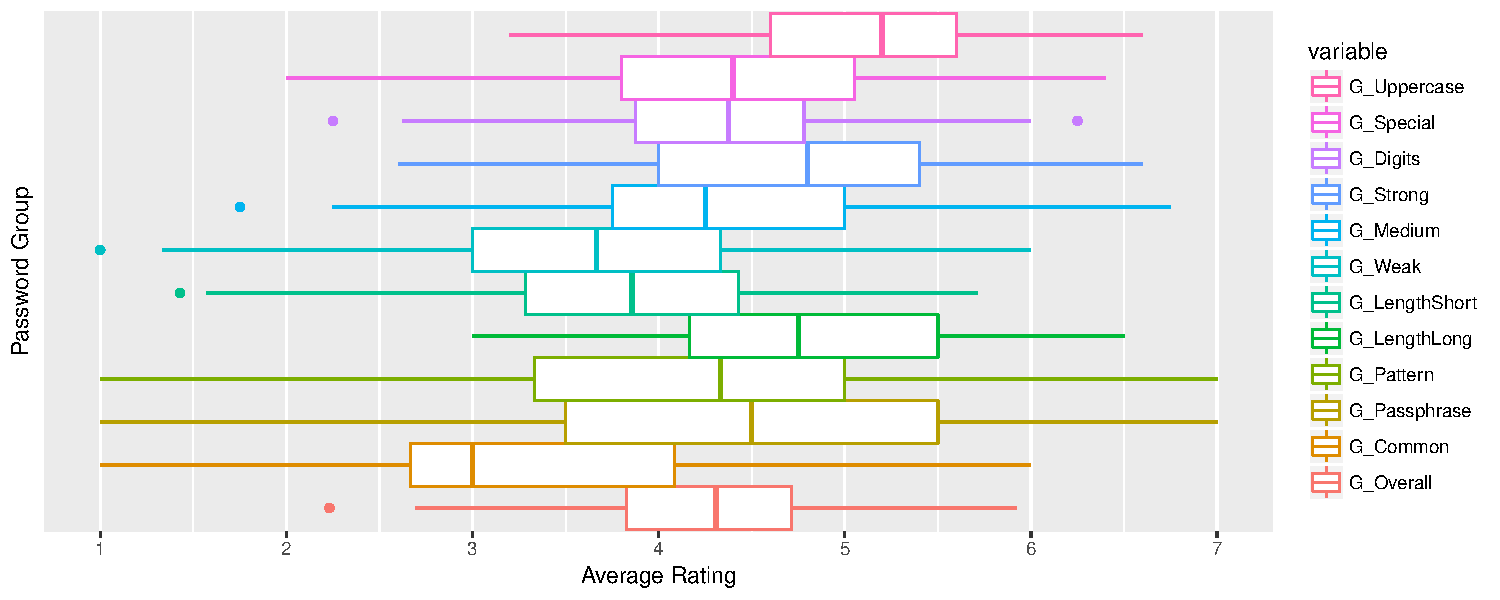
\includegraphics[width=\linewidth]{personality/avearge-rating-boxplot}
	\caption{\label{fig:personality:study2:average-rating-boxplot}}
\end{figure}

%%%%%% TABLE 
%\begin{table*}%[h!tbp]
  \small
  \centering
  \caption{Regression analysis for password ratings in different categories as dependent variables and psychometrics as independent variables variables. Demographic data serves as control variables. Numbers in bold indicate statistical significance ($p<0.05$). The Big-Five factors had higher predictive value and than the GMDS factors.}
    \resizebox{\linewidth}{!}
{
\begin{tabular}{rl|r|rr|rrr|rrr}
    \multicolumn{2}{l|}{Predictor} & \multicolumn{1}{l|}{Overall} & \multicolumn{1}{l}{Short} & \multicolumn{1}{l|}{Long} & \multicolumn{1}{l}{Weak} & \multicolumn{1}{l}{Medium} & \multicolumn{1}{l|}{Strong} & \multicolumn{1}{l}{Symbols} & \multicolumn{1}{l}{Digits} & \multicolumn{1}{l}{Uppercase} \\
\cmidrule{3-11}    \rowcolor[rgb]{ .718,  .871,  .91} \multicolumn{1}{l}{Big Five} & Neuroticism & \cellcolor[rgb]{ 1,  1,  1}  & \cellcolor[rgb]{ .949,  .91,  .518} 0.15 & \cellcolor[rgb]{ .949,  .91,  .518} 0.15 & \cellcolor[rgb]{ .969,  .914,  .518} 0.14 & \cellcolor[rgb]{ 1,  1,  1}  & \cellcolor[rgb]{ .98,  .627,  .459} -0.15 & \cellcolor[rgb]{ 1,  1,  1}  & \cellcolor[rgb]{ 1,  1,  1}  & \cellcolor[rgb]{ 1,  1,  1}  \\
    \rowcolor[rgb]{ .718,  .871,  .91}   & Openness & \cellcolor[rgb]{ .976,  .518,  .439} \textbf{-0.25} & \cellcolor[rgb]{ .976,  .541,  .443} \textbf{-0.23} & \cellcolor[rgb]{ .98,  .573,  .447} \textbf{-0.2} & \cellcolor[rgb]{ .976,  .498,  .435} \textbf{-0.27} & \cellcolor[rgb]{ .98,  .616,  .459} -0.16 & \cellcolor[rgb]{ .98,  .604,  .455} -0.17 & \cellcolor[rgb]{ .984,  .647,  .463} -0.13 & \cellcolor[rgb]{ .976,  .541,  .443} \textbf{-0.23} & \cellcolor[rgb]{ .984,  .639,  .463} -0.14 \\
    \rowcolor[rgb]{ .718,  .871,  .91}   & Agreeableness & \cellcolor[rgb]{ .898,  .894,  .514} 0.18 & \cellcolor[rgb]{ .949,  .91,  .518} 0.15 & \cellcolor[rgb]{ .898,  .894,  .514} 0.18 & \cellcolor[rgb]{ .898,  .894,  .514} 0.18 & \cellcolor[rgb]{ 1,  1,  1}  & \cellcolor[rgb]{ .969,  .914,  .518} 0.14 & \cellcolor[rgb]{ .984,  .918,  .518} 0.13 & \cellcolor[rgb]{ .996,  .91,  .514} 0.11 & \cellcolor[rgb]{ 1,  1,  1}  \\
    \rowcolor[rgb]{ .988,  .835,  .706} \multicolumn{1}{l}{GDMS} & Rational & \cellcolor[rgb]{ 1,  1,  1}  & \cellcolor[rgb]{ 1,  1,  1}  & \cellcolor[rgb]{ 1,  1,  1}  & \cellcolor[rgb]{ 1,  1,  1}  & \cellcolor[rgb]{ 1,  1,  1}  & \cellcolor[rgb]{ 1,  1,  1}  & \cellcolor[rgb]{ 1,  1,  1}  & \cellcolor[rgb]{ 1,  1,  1}  & \cellcolor[rgb]{ .984,  .918,  .518} 0.13 \\
    \rowcolor[rgb]{ .988,  .835,  .706}   & Intuitive & \cellcolor[rgb]{ 1,  1,  1}  & \cellcolor[rgb]{ 1,  1,  1}  & \cellcolor[rgb]{ 1,  1,  1}  & \cellcolor[rgb]{ 1,  1,  1}  & \cellcolor[rgb]{ 1,  1,  1}  & \cellcolor[rgb]{ 1,  1,  1}  & \cellcolor[rgb]{ 1,  1,  1}  & \cellcolor[rgb]{ 1,  1,  1}  & \cellcolor[rgb]{ .996,  .898,  .51} 0.1 \\
    \rowcolor[rgb]{ .988,  .835,  .706}   & Avoidant & \cellcolor[rgb]{ 1,  1,  1}  & \cellcolor[rgb]{ 1,  1,  1}  & \cellcolor[rgb]{ 1,  1,  1}  & \cellcolor[rgb]{ .984,  .639,  .463} -0.14 & \cellcolor[rgb]{ 1,  1,  1}  & \cellcolor[rgb]{ 1,  1,  1}  & \cellcolor[rgb]{ .984,  .647,  .463} -0.13 & \cellcolor[rgb]{ 1,  1,  1}  & \cellcolor[rgb]{ 1,  1,  1}  \\
    \rowcolor[rgb]{ .988,  .835,  .706}   & Spontaneous & \cellcolor[rgb]{ 1,  1,  1}  & \cellcolor[rgb]{ 1,  1,  1}  & \cellcolor[rgb]{ 1,  1,  1}  & \cellcolor[rgb]{ 1,  1,  1}  & \cellcolor[rgb]{ .984,  .918,  .518} 0.13 & \cellcolor[rgb]{ 1,  1,  1}  & \cellcolor[rgb]{ .949,  .91,  .518} 0.15 & \cellcolor[rgb]{ 1,  1,  1}  & \cellcolor[rgb]{ 1,  1,  1}  \\
      & Education &   & \cellcolor[rgb]{ .914,  .898,  .514} 0.17 &   & \cellcolor[rgb]{ .984,  .918,  .518} 0.13 & \cellcolor[rgb]{ 1,  .922,  .518} 0.12 &   &   & \cellcolor[rgb]{ .933,  .902,  .514} 0.16 &  \\
      & CS Background & \cellcolor[rgb]{ .984,  .647,  .463} -0.13 &   & \cellcolor[rgb]{ .984,  .647,  .463} -0.13 &   & \cellcolor[rgb]{ .98,  .627,  .459} -0.15 & \cellcolor[rgb]{ .984,  .682,  .471} -0.1 &   & \cellcolor[rgb]{ .984,  .682,  .471} -0.1 &  \\
    \midrule
      & F & 4.23 & 2.83 & 3.54 & 3.46 & 1.9 & 2.48 & 1.91 & 2.52 & 1.19 \\
      & df & 3 & 4 & 4 & 5 & 4 & 4 & 4 & 4 & 3 \\
      & p & < 0.01 & < 0.05 & < 0.05 & < 0.01 & > 0.1 & < 0.05 & > 0.1 & < 0.05 & > 0.1 \\
      & R$^2$ & \cellcolor[rgb]{ .761,  .898,  .804} 0.12 & \cellcolor[rgb]{ .788,  .91,  .827} 0.11 & \cellcolor[rgb]{ .733,  .886,  .78} 0.13 & \cellcolor[rgb]{ .675,  .863,  .729} 0.15 & \cellcolor[rgb]{ .906,  .957,  .929} 0.07 & \cellcolor[rgb]{ .82,  .922,  .855} 0.1 & \cellcolor[rgb]{ .906,  .957,  .929} 0.07 & \cellcolor[rgb]{ .82,  .922,  .855} 0.1 & \cellcolor[rgb]{ .988,  .988,  1} 0.04 \\
      & Adjusted R$^2$ & \cellcolor[rgb]{ .706,  .875,  .757} 0.09 & \cellcolor[rgb]{ .776,  .906,  .82} 0.07 & \cellcolor[rgb]{ .706,  .875,  .757} 0.09 & \cellcolor[rgb]{ .635,  .847,  .698} 0.11 & \cellcolor[rgb]{ .882,  .949,  .91} 0.04 & \cellcolor[rgb]{ .812,  .918,  .851} 0.06 & \cellcolor[rgb]{ .918,  .961,  .941} 0.03 & \cellcolor[rgb]{ .812,  .918,  .851} 0.06 & \cellcolor[rgb]{ .988,  .988,  1} 0.01 \\
    \bottomrule
    \bottomrule
    \end{tabular}%
}
  \label{tab:Regression-Rating}%
\end{table*}%

%%%%%%%%%%%%%%%%%%%%%%%%%%
%%% 
%%% 		STRENGTH RATING
%%% 
%%%%%%%%%%%%%%%%%%%%%%%%%%
\subsubsection{Standalone Strength Rating}
Next, we analyze associations between personality and password perception. Internal consistency of the scale was fair (Cronbach's $\alpha=0.72$). 
%TODO marginal effects first, then combine the most important covariates in a smooth term (s(x, y))

\paragraph{Model 1: Big-Five Scores with minimal REML smoothing}
For overall strength rating, most covariates revealed linear associations (Table \ref{tab:appendix:gam-overall-rating-reml} in the Appendix lists the coefficients). In Figure \ref{fig:personality:study2:rating-b5-predictors-G_Overall}, we see that participants who scored higher on the \textit{openness} trait generally judged passwords lower. This effect was flagged as significant in the model ($B=-0.36, \beta=-0.25$). For \textit{agreeableness}, we can see a slightly more positive trend, i.e. participants tended to rate passwords higher, the higher they scored on the \textit{agreeableness} scale. The other traits did not show any conclusive association. Having a computer-science background revealed slightly lower assessments ($B=-2.92, \beta=-0.14$), but the association was not significant. The model fit was rather low with \Rsqadj{0.06} and an explained deviance of 14.7\%. Associations and model fits were comparable for the ``short password'' and ``weak password'' categories. The highest model fit was achieved for the ``Passphrase'' category (\Rsqadj{0.17}, explained deviance 26.3\%), suggesting that passphrases were largely responsible for the overall strength rating model. In summary, personality did not explain much of the participants' assessment. Penalizing smoothing parameters in stronger ways achieved higher model fits, however, the likelihood of overfitting the models increases. Therefore, we explored different factor constellations to get closer to explaining strength perceptions.

\begin{figure}[htbp]
	\centering
	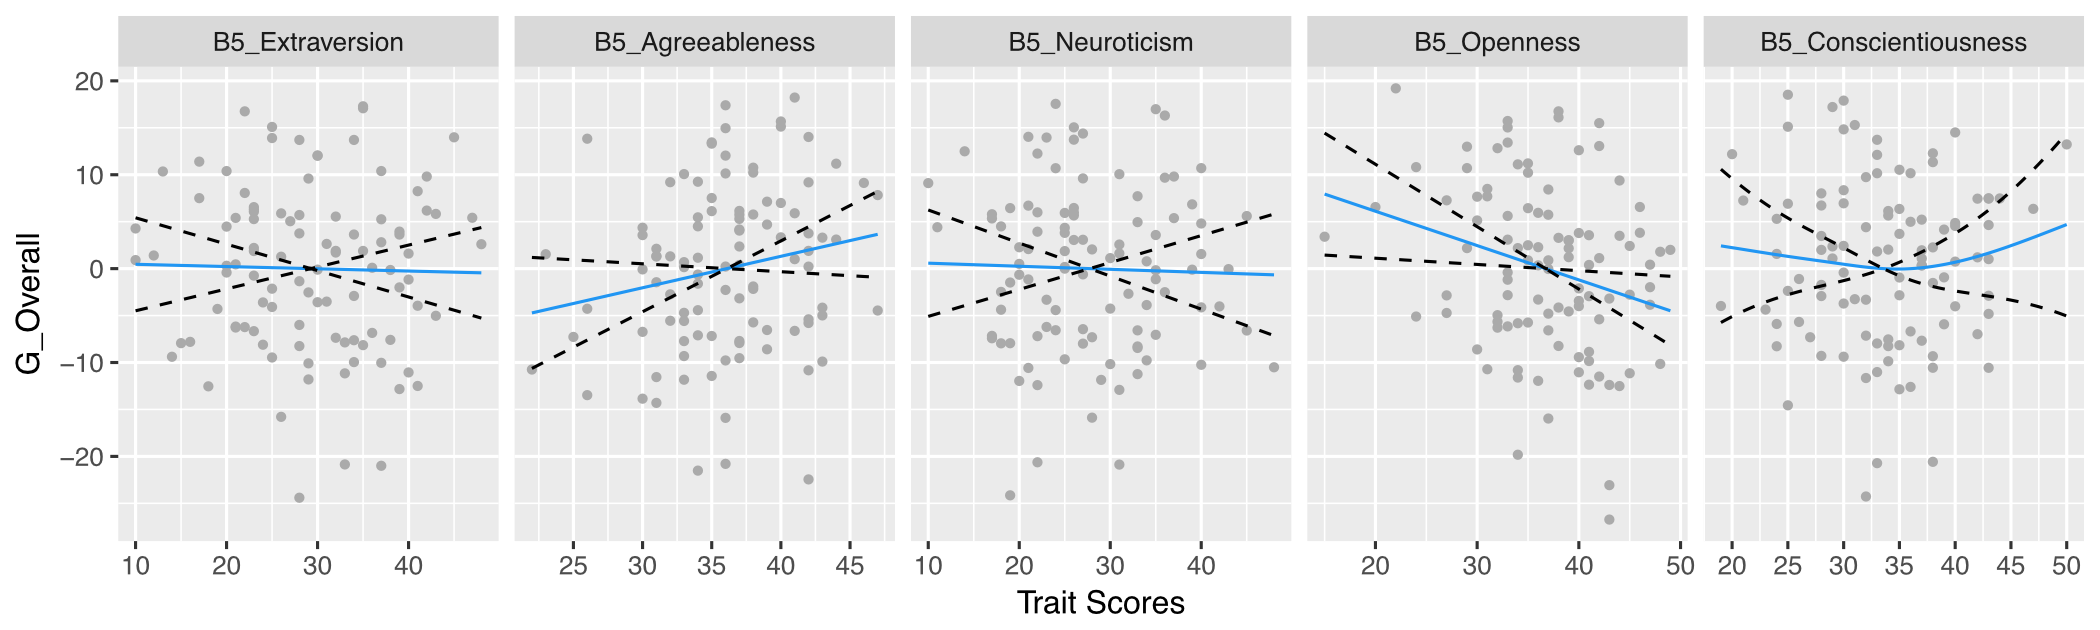
\includegraphics[width=\linewidth]{personality/rating-b5-predictors-G_Overall}
	\caption{\label{fig:personality:study2:rating-b5-predictors-G_Overall}Visualization of generalized additive models for overall strength perceptions (i.e. tendency to judge a password stronger) with Big-Five traits as covariates. There is a significant negative association for openness: participants scoring higher on the openness trait judged password strength lower.}
\end{figure}


\paragraph{Model 2: Extracted Factors as Predictors}
Although the IPIP scale showed good internal consistency, we can try to break down the contributing factors. Usually, a \textit{Principal Component Analysis} (PCA) reduces the number of factors, but does not have to. In our case, we would expect five distinct factors from the 50 items, but a PCA revealed that there might be \textbf{ten} for our data set. We thus extracted those factors with a standard factor analysis using varimax rotation and used these factors as predictors instead of the big-five trait scores. The resulting model explained a larger portion of the deviance (20.1\% vs. 14.7\%) for overall assessment, but the R-square value remained constant. Coefficients for Factor 3 were biggest ($B=-2.16, \beta=-0.21$), and all items of the openness sub-scale loaded onto it. To a much smaller degree, conscientiousness, agreeableness, and extraversion items also formed this factor. As a consequence, marginal effects, i.e. caused by only one personality trait, can be ruled out -- it is a combination of trait scores that explains associations in our model. However, only a confirmatory study with a larger sample size can deliver final answers as to the specific trait combinations. As of now, we hypothesize that participants showing particular constellations of openness, conscientiousness and extraversion scores rated all passwords lower than other participants.
\begin{figure}[htbp]
	\centering
	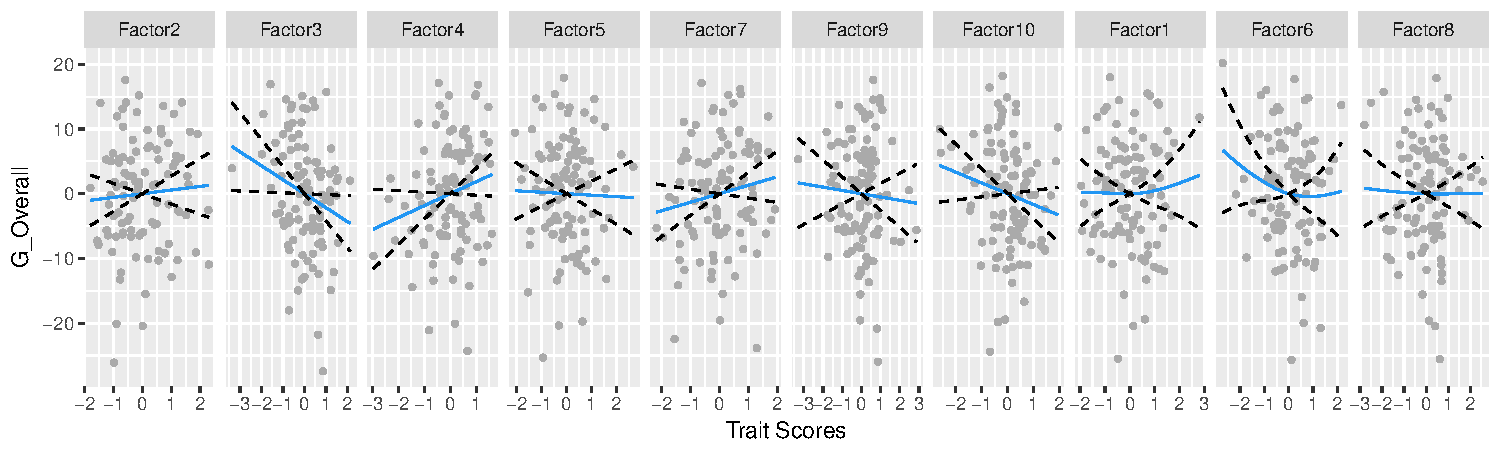
\includegraphics[width=\linewidth]{personality/rating-fa-predictors-G_Overall}
	\caption{\label{fig:personality:study2:rating-fa-predictors-G_Overall}A principal component analysis suggested there might be 10 explanatory factors in our dataset for the personality construct, which we then extracted using varimax rotation. Factor 3, which was mostly loaded with \textit{openness} items, Factor 9 (mostly \textit{conscientiousness}), and Factor 10 (mostly \textit{extraversion}) were associated with lower ratings.}
\end{figure}

\paragraph{Model 3: Mixed Model -- Password Characteristics and Big Five Traits}
Similar to the evaluation of PASDJO strength ratings, we can take the different features of the passwords as covariates, e.g. the number of digits or the total length. Figure \ref{fig:personality:study2:boxplot-ratings-pws} visualizes the ratings for each password. We see that strength ratings take a broad score spectrum in many cases, with the exception of those passwords that contained symbols. Using password features as covariates allows us to identify their weight in the assessment. 

\begin{figure}[htbp]
	\centering
	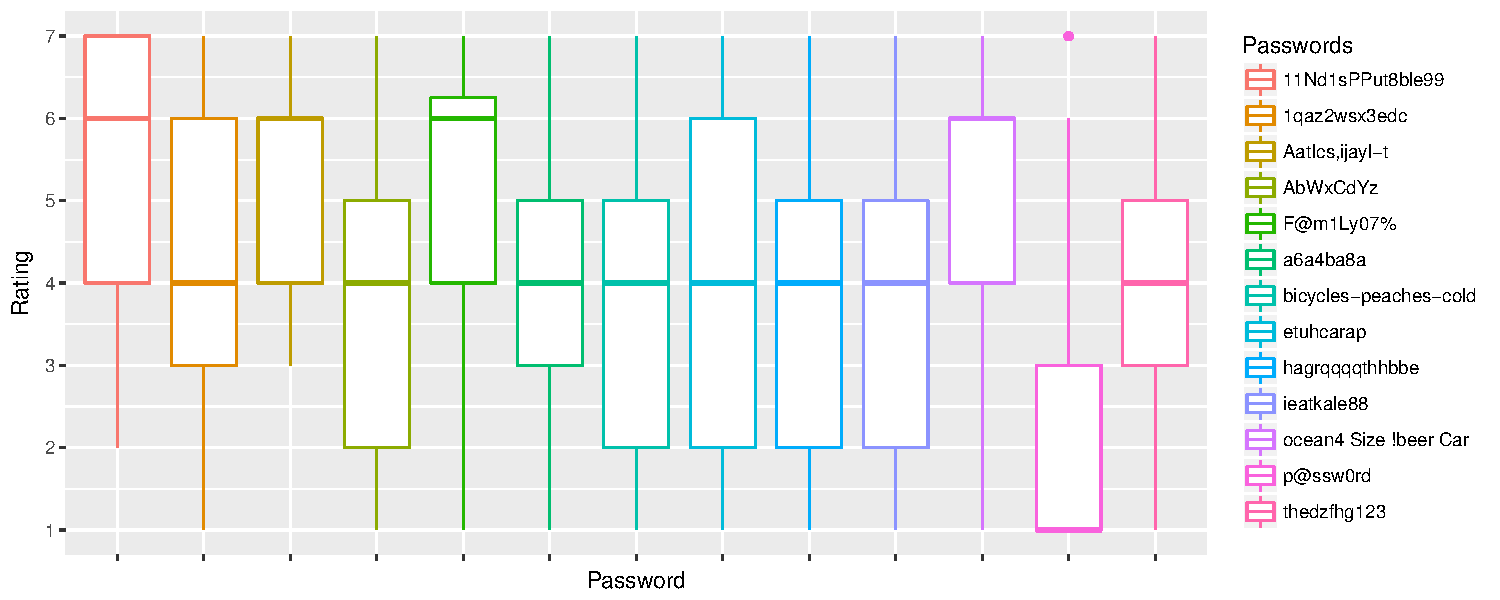
\includegraphics[width=\linewidth]{personality/boxplot-ratings-pws-v2}
	\caption{\label{fig:personality:study2:boxplot-ratings-pws}Participants' subjective strength assessments of the 13 passwords in the study. Broad interquartile ranges for indicate that participants largely disagreed on the strength.}
\end{figure}

\makeatletter
First, we look at marginal associations between ratings and the number of lowercase, uppercase, digits, and symbols (LUDS metric), which is basically a linear model. All coefficients are positive ($\beta_{L} = 0.15$, $\beta_{U} = 0.24$,$\beta_{D} = 0.26$,$\beta_{S} = 0.13$) but weakly associated, and the model fit is rather low (\Rsqadj{0.12}). Mixing it with the Big-Five traits as predictors improves the fit slightly (\Rsqadj{0.15}). If we factor in \textit{password length} as an interaction term with the LUDS metrics, the fit improves further (\Rsqadj{0.20}). The correlation between the number of digits and ratings becomes strong ($\beta_{L} = 0.84$), i.e. more digits are perceived as stronger. This, however, was surprisingly contradicted when we account for the fact that two passwords had digits as substitutions for letters (\textit{p@ssw0rd} and \textit{F@m1Ly07\%}). Thus, the final model includes an interaction term $digits*substitutions*symbols$ as covariate and achieves the best model fit overall (\Rsqadj{0.25}). In Figure \ref{fig:personality:study2:rating-mixed-model} we can see the resulting associations. Password length was the primary factor, while the influence of character substitutions reversed the positive impression of symbols, digits and uppercase characters.
%what about Big five? 
Personality traits on the other side, although statistically significant, were weak predictors. However, removing them from the model entirely would have led to a notable decrease in model fit ($\Delta=0.05$). 

\paragraph{Conclusion} The mixed model is strongly influenced by interaction terms with predictable character substitutions. In general, more digits, uppercase letters, and symbols led to higher strength ratings, but this association was strongly reversed if digits or symbols acted as l33t substitutions. Thus, we conclude that respondents were skeptical about this password creation strategy in the rating part. By and large, personality was a minor factor.

% weird: including the number of substitutions flips the direction of the correlation: but since only p@ssw0rd and F@m1Ly07% had numbers and substitutions, this means that people penalized these two passwords. 

\begin{figure}[htbp]
	\centering
	\begin{subfigure}[t]{\linewidth}
		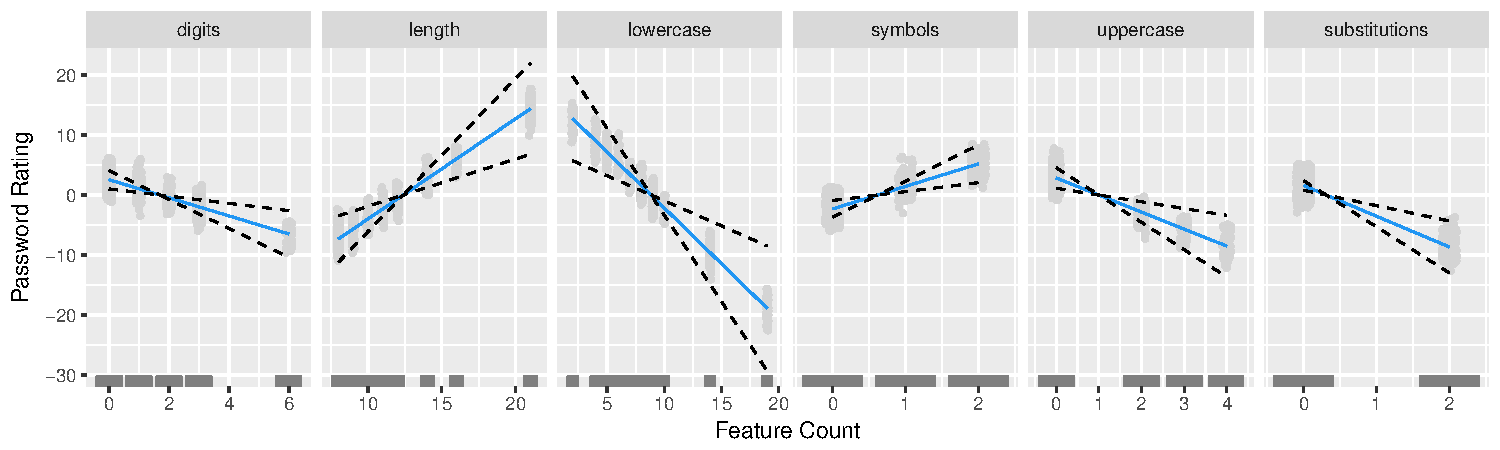
\includegraphics[width=\textwidth]{personality/rating-manual-mixed-v9-predictors}
	\end{subfigure}
	\begin{subfigure}[b]{\linewidth}
	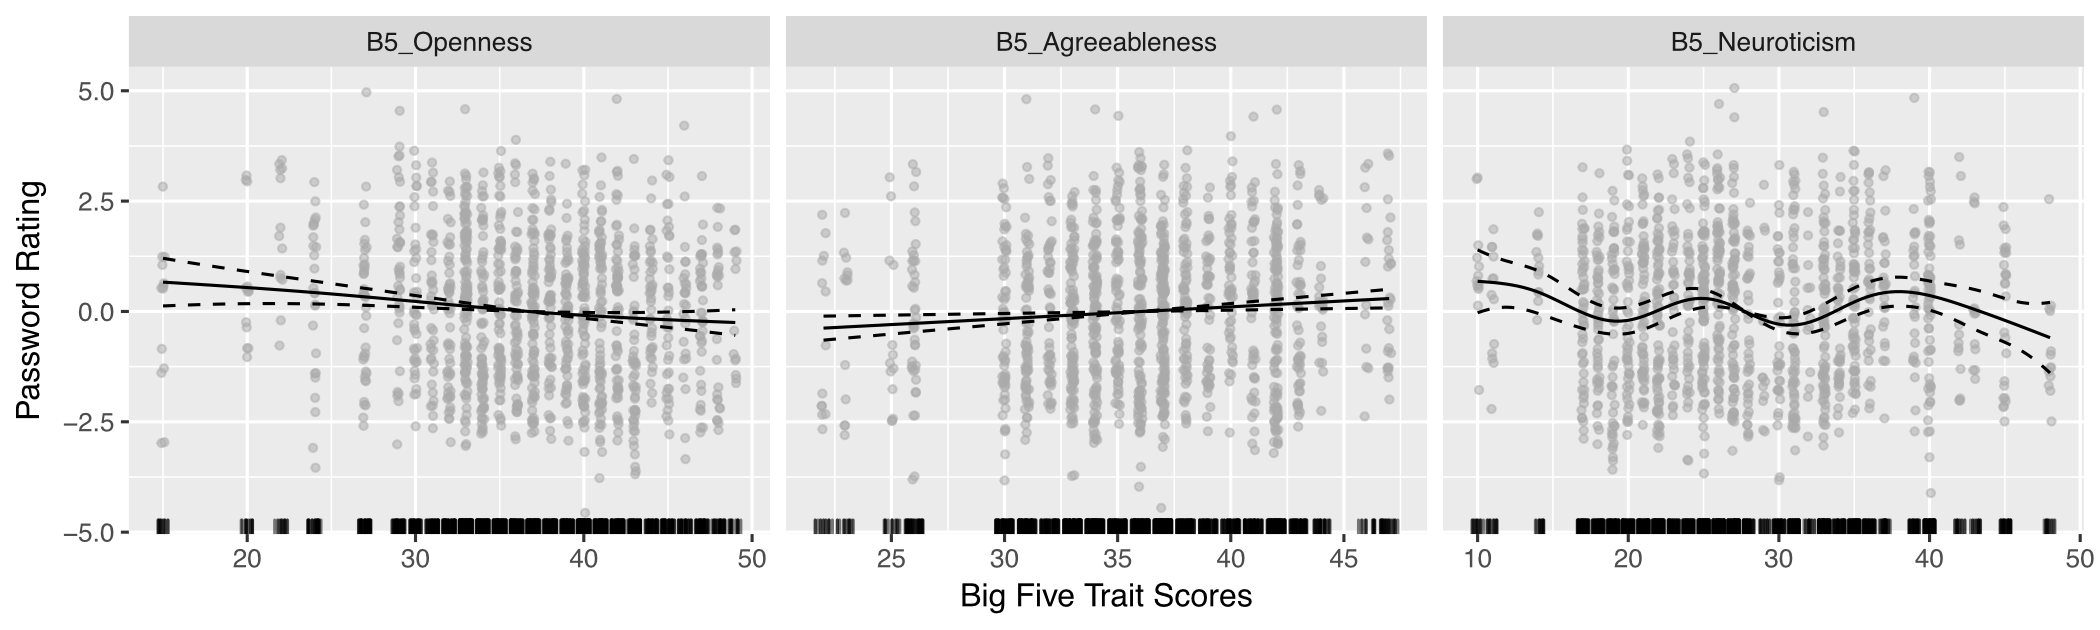
\includegraphics[width=\textwidth]{personality/rating-manual-mixed-v9-b5}
	\end{subfigure}
	\caption{\label{fig:personality:study2:rating-mixed-model} Top: Longer passwords were perceived as stronger. Correlations turned negative if, substitutions were factored into the model. Bottom: Personality traits showed very small associations.}
\end{figure}

%%%%%%%%%%%%%%%%%%%%%%%%%%
%%% 
%%% 		META PASSWORD
%%% 
%%%%%%%%%%%%%%%%%%%%%%%%%%
\subsubsection{Standalone ratings modeled with Meta password}
Trying to understand if participants' past behavior might have influenced their judgment, we created GAMs analogously with metrics of their \textit{meta password}. The only notable association, which was conclusive across the board, was the reported number of uppercase characters. We found that with increasing usage of uppercase letters, participants tended to give lower ratings ($\beta=-0.27$). 

%%%%%%%%%%%%%%%%%%%%%%%%%%
%%% 
%%% 		STRENGTH COMPARISON
%%% 
%%%%%%%%%%%%%%%%%%%%%%%%%%
\subsubsection{Comparisons Between Two Passwords}

We explored whether personality traits influence how participants decide between two given passwords. We modeled the comparison on the 7-point scale such that 1 represents a vote against a feature and 7 for a feature, e.g. more digits. Only conscientiousness was retained as predictor in all models. The most interesting association was found when one of the two passwords contained digits: Choosing the password with more digits positively correlated with higher conscientiousness scores ($\beta = 0.43$). The opposite is true for participants scoring high on the openness scale. They are more likely to vote for the longer password (non linearly) than for the one containing digits ($\beta = -0.17$). Totaling up all character classes used in a password, we see that the more diverse it was, the more likely it was favored by participants with high conscientiousness scores ($\beta = 0.36$). 
%control
In this particular model, there were weak associations between gender and character diversity. Male participants were more likely to prefer the password consisting of more character classes ($\beta = 0.23$). Having a computer-science background correlated with preference for the longer password ($\beta = 0.21$).

In all the models, the predictive power was moderate and did not reach the levels from Model 3 in the rating task. However, the correlation coefficients were stronger for personality trait. We find that the decision between two given passwords is mostly associated with the conscientiousness and openness traits.



%%regression comparison

% Table generated by Excel2LaTeX from sheet 'Latex Separate Regressions'
\begin{table*}[h]
 \centering
 \small
  \caption{Regression analysis of the comparison task. Conscientiousness and openness are the most important predictors. Open participants were more likely to vote for the longer password instead of the one with digits, while the inverse is true for conscientious participants. Rational decision makers failed to identify the stronger password more often.}
             \begin{tabular}{rl|rr|rrrr}
      & Predictor & \multicolumn{1}{l}{Length} & \multicolumn{1}{l|}{Strength} & \multicolumn{1}{l}{Symbols} & \multicolumn{1}{l}{Digits} & \multicolumn{1}{l}{Cases} & \multicolumn{1}{l}{Classes} \\
\cmidrule{3-8}    \rowcolor[rgb]{ .718,  .871,  .91} \multicolumn{1}{l}{Big Five} & Neuroticism & \cellcolor[rgb]{ 1,  1,  1}  & \cellcolor[rgb]{ .98,  .627,  .459} -0.15 & \cellcolor[rgb]{ 1,  1,  1}  & \cellcolor[rgb]{ .878,  .89,  .514} 0.19 & \cellcolor[rgb]{ 1,  1,  1}  & \cellcolor[rgb]{ 1,  1,  1}  \\
    \rowcolor[rgb]{ .718,  .871,  .91}   & Extraversion & \cellcolor[rgb]{ 1,  1,  1}  & \cellcolor[rgb]{ .98,  .596,  .455} -0.18 & \cellcolor[rgb]{ 1,  1,  1}  & \cellcolor[rgb]{ 1,  1,  1}  & \cellcolor[rgb]{ 1,  1,  1}  & \cellcolor[rgb]{ 1,  1,  1}  \\
    \rowcolor[rgb]{ .718,  .871,  .91}   & Openness & \cellcolor[rgb]{ .741,  .847,  .506} \textbf{0.27} & \cellcolor[rgb]{ .914,  .898,  .514} 0.17 & \cellcolor[rgb]{ 1,  1,  1}  & \cellcolor[rgb]{ .976,  .541,  .443} \textbf{-0.23} & \cellcolor[rgb]{ 1,  1,  1}  & \cellcolor[rgb]{ .984,  .671,  .467} -0.11 \\
    \rowcolor[rgb]{ .718,  .871,  .91}   & Agreeableness & \cellcolor[rgb]{ .969,  .914,  .518} 0.14 & \cellcolor[rgb]{ .996,  .91,  .514} 0.11 & \cellcolor[rgb]{ 1,  1,  1}  & \cellcolor[rgb]{ 1,  1,  1}  & \cellcolor[rgb]{ 1,  1,  1}  & \cellcolor[rgb]{ 1,  1,  1}  \\
    \rowcolor[rgb]{ .718,  .871,  .91}   & Conscientiousness & \cellcolor[rgb]{ .984,  .659,  .467} -0.12 & \cellcolor[rgb]{ .898,  .894,  .514} 0.18 & \cellcolor[rgb]{ .969,  .914,  .518} 0.14 & \cellcolor[rgb]{ .388,  .745,  .482} \textbf{0.47} & \cellcolor[rgb]{ .878,  .89,  .514} 0.19 & \cellcolor[rgb]{ .635,  .816,  .498} \textbf{0.33} \\
    \rowcolor[rgb]{ .988,  .835,  .706} \multicolumn{1}{l}{GDMS} & Rational & \cellcolor[rgb]{ .976,  .486,  .431} \textbf{-0.28} & \cellcolor[rgb]{ .973,  .412,  .42} \textbf{-0.35} & \cellcolor[rgb]{ 1,  1,  1}  & \cellcolor[rgb]{ .898,  .894,  .514} 0.18 & \cellcolor[rgb]{ 1,  1,  1}  & \cellcolor[rgb]{ 1,  1,  1}  \\
    \rowcolor[rgb]{ .988,  .835,  .706}   & Intuitive & \cellcolor[rgb]{ .98,  .627,  .459} -0.15 & \cellcolor[rgb]{ .98,  .596,  .455} -0.18 & \cellcolor[rgb]{ 1,  1,  1}  & \cellcolor[rgb]{ 1,  1,  1}  & \cellcolor[rgb]{ 1,  1,  1}  & \cellcolor[rgb]{ 1,  1,  1}  \\
    \rowcolor[rgb]{ .988,  .835,  .706}   & Dependent & \cellcolor[rgb]{ 1,  1,  1}  & \cellcolor[rgb]{ 1,  1,  1}  & \cellcolor[rgb]{ 1,  1,  1}  & \cellcolor[rgb]{ 1,  1,  1}  & \cellcolor[rgb]{ .984,  .918,  .518} 0.13 & \cellcolor[rgb]{ 1,  1,  1}  \\
    \rowcolor[rgb]{ .988,  .835,  .706}   & Avoidant & \cellcolor[rgb]{ 1,  1,  1}  & \cellcolor[rgb]{ 1,  1,  1}  & \cellcolor[rgb]{ .984,  .659,  .467} -0.12 & \cellcolor[rgb]{ .827,  .875,  .51} 0.22 & \cellcolor[rgb]{ 1,  1,  1}  & \cellcolor[rgb]{ 1,  1,  1}  \\
    \rowcolor[rgb]{ .988,  .835,  .706}   & Spontaneous & \cellcolor[rgb]{ 1,  1,  1}  & \cellcolor[rgb]{ 1,  1,  1}  & \cellcolor[rgb]{ 1,  1,  1}  & \cellcolor[rgb]{ 1,  1,  1}  & \cellcolor[rgb]{ .98,  .616,  .459} -0.16 & \cellcolor[rgb]{ 1,  1,  1}  \\
      & Education &   &   &   & \cellcolor[rgb]{ .984,  .659,  .467} -0.12 &   &  \\
      & CS Background & \cellcolor[rgb]{ .843,  .878,  .51} \textbf{0.21} & \cellcolor[rgb]{ .843,  .878,  .51} \textbf{0.21} &   & \cellcolor[rgb]{ .984,  .682,  .471} -0.1 &   &  \\
      & Male &   &   & \cellcolor[rgb]{ .843,  .878,  .51} \textbf{0.21} & \cellcolor[rgb]{ .949,  .91,  .518} 0.15 & \cellcolor[rgb]{ .706,  .839,  .502} \textbf{0.29} & \cellcolor[rgb]{ .843,  .878,  .51} \textbf{0.21} \\
    \midrule
      & F & 3.95 & 3.78 & 3.37 & 3.13 & 3.86 & 5.75 \\
      & df & 6 & 8 & 3 & 8 & 4 & 3 \\
      & p & \multicolumn{1}{l}{< 0.01} & \multicolumn{1}{l|}{< 0.01} & \multicolumn{1}{l}{< 0.05} & \multicolumn{1}{l}{< 0.01} & \multicolumn{1}{l}{< 0.01} & \multicolumn{1}{l}{<0.01} \\
      & R$^2$ & \cellcolor[rgb]{ .533,  .804,  .608} 0.2 & \cellcolor[rgb]{ .388,  .745,  .482} 0.25 & \cellcolor[rgb]{ .82,  .922,  .855} 0.1 & \cellcolor[rgb]{ .506,  .792,  .584} 0.21 & \cellcolor[rgb]{ .706,  .875,  .757} 0.14 & \cellcolor[rgb]{ .675,  .863,  .729} 0.15 \\
      & Adjusted R$^2$& \cellcolor[rgb]{ .494,  .788,  .576} 0.15 & \cellcolor[rgb]{ .388,  .745,  .482} 0.18 & \cellcolor[rgb]{ .776,  .906,  .82} 0.07 & \cellcolor[rgb]{ .494,  .788,  .576} 0.15 & \cellcolor[rgb]{ .671,  .863,  .729} 0.1 & \cellcolor[rgb]{ .565,  .82,  .635} 0.13 \\
    \bottomrule
    \bottomrule
    \end{tabular}%
  \label{tab:Comparison-Regression}%
\end{table*}%


\subsubsection{Qualitative Findings}
While entering an elaborate response as to the judgment approach was not mandatory, all but one participant (\textit{n}=99) gave a brief and in most cases comprehensible explanation for their ratings. The following numbers do not necessarily add up to \textit{n}, because an answer could contain multiple codes.

We identified four overall themes in how the participants approached rating passwords: \textit{Character diversity}, \textit{creation strategy}, \textit{predictability} and \textit{other}. The character diversity code consists of participants mentioning the importance of symbols (69), digits (52), upper-/lowercase letters (45) and general variety of characters (16). Regarding the creation strategy, many participants penalized passwords when they contained actual words (40) or personal information (3). The predictability category was divided into answers referring to character substitutions (10), patterns (17), guessability (12), randomness (20), length (25) and the position of symbols/digits (6). The other themes were established from 8 participants using technical jargon (e.g. ``attack'' or ``brute force'') and those who identified the obfuscated passwords (2). These themes echo the quantitative ratings very well. 

\subsection{Finding Summary}
We found that participants evaluate password strength by looking for specific patterns. Regression models and qualitative analysis show that respondents mostly penalized lack of diversity and randomness which is consistent with related work \cite{Ur2016PerceptionsPassword}. Thus, the associations originating from different personality traits were small in many cases, but not negligible. Technical background and gender played a role in the comparison task, because male participants were more likely influenced by character diversity. On aggregate, the predictive power of the independent variables was higher in the comparison task than in the standalone rating. Nonetheless, a fine-grained mixed model revealed interesting side effects for standalone ratings. These include the reversal of the correlation if a digit or symbol was used to substitute a letter. The most important personality factors across both tasks were \textbf{openness}, \textbf{agreeableness} and \textbf{conscientiousness}. The sample size might have been too small to yield narrow confidence intervals and impressive model fits. As exploratory stage, however, the data provides considerable evidence as to the feasibility of investigating ``password personality''. 